\section{Platform}

\begin{frame}
\frametitle{Kriterier}
Baseret på metaforen "f-16 fly"
\begin{itemize}
\item Modulær
\item Fleksibel
\item Kombinerbar
\item Kommunikativ
\end{itemize}
\end{frame}

\begin{frame}
\frametitle{Arkitektur}
\begin{figure}[h]
	\centering						%  l   b   r	t
	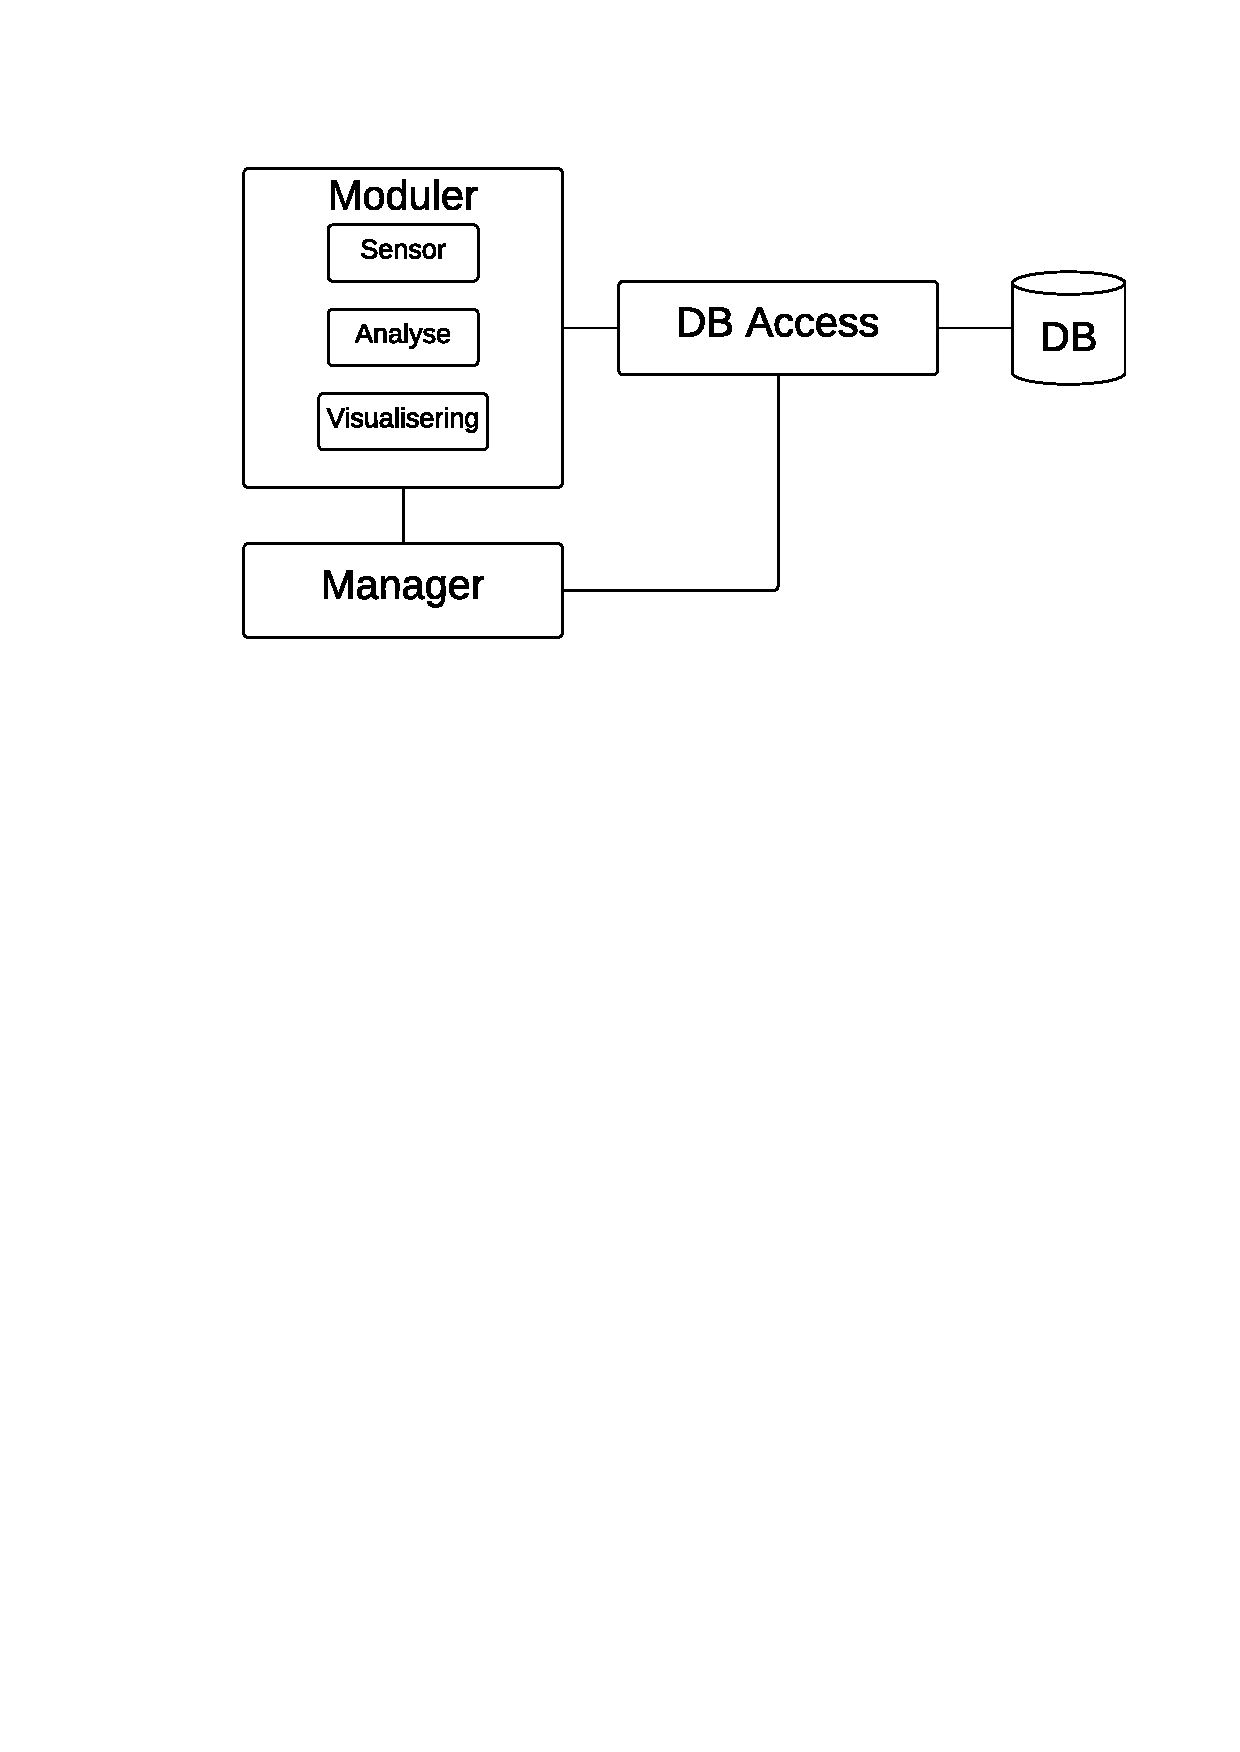
\includegraphics[scale=0.5, trim = 1cm 17.5cm 1cm 1cm, clip]{graphics/ArkitekturLucidChart}
	\caption{Systemets arkitektur}
  \label{arkitektur_udkast_1}
\end{figure}
\end{frame}

\begin{frame}
\frametitle{arkitektur - DB}
\begin{itemize}
\item Data fra alle moduler
\end{itemize}
\end{frame}

\begin{frame}
\frametitle{arkitektur - DB Access}
\begin{itemize}
\item Adgangslag til DB
\item Muliggør abstraktion over data lokation
\end{itemize}
\end{frame}

\begin{frame}
\frametitle{arkitektur - Moduler}
\begin{itemize}
\item 3 typer
\begin{itemize}
\item Data
\item Analyse
\item Visning
\end{itemize}
\item Hver kan bruge data fra de andre
\end{itemize}
\end{frame}

\begin{frame}
\frametitle{arkitektur - Manager}
\begin{itemize}
\item Central kontrol enhed
\item Del brugeren interagerer med
\item Kontrollerer hvilke moduler der skal køre 
\end{itemize}
\end{frame}

\begin{frame}
\frametitle{Arkitektur - Kriterier}
Kriterierne dækkes af følgende elementer i arkitekturen:
\begin{itemize}
\item Modulær -> Moduler
\item Fleksibel -> Manager
\item Kombiner -> Moduler
\item Kommunikativ -> DB Access/DB
\end{itemize}
\end{frame}

\begin{frame}
\frametitle{Eksempel}
\begin{itemize}
\item Krav til start på modul navn
\begin{itemize}
\item dk.cs.aau.psylog.sensor
\item dk.cs.aau.psylog.analysis
\item dk.cs.aau.psylog.view
\end{itemize}
\item Valid JSON-skema(Bilag D)
\end{itemize}
\end{frame}

